\documentclass[aspectratio=149]{beamer}
\usepackage[utf8]{inputenc}

\usepackage[utf8]{inputenc}
\usepackage[T1]{fontenc}

\usepackage[english]{babel}
\usepackage{amsmath}
\usepackage{cleveref}
\usepackage{amssymb}
\usepackage{mathtools}

%%Numbers, expectation
\newcommand{\N}{\mathbb{N}}
\newcommand{\E}{\mathbb{E}}
\renewcommand{\P}{\mathbb{P}}
\newcommand{\Var}{\mathbb{V}}
\newcommand{\R}{\mathbb{R}}
\newcommand{\D}{\mathcal{D}}
\newcommand{\B}{\mathcal{B}}
\newcommand{\Dh}{\D_h}
\renewcommand{\phi}{\varphi}
\newcommand*\diff{\mathop{}\!\mathrm{d}} % integral

%% mathoperator
\DeclareMathOperator*{\argmax}{arg\,max}
\DeclareMathOperator*{\argmin}{arg\,min}
\DeclareMathOperator*{\dom}{dom}
\DeclareMathOperator*{\sign}{sign}
\DeclareMathOperator*{\diag}{diag}

\DeclareMathOperator*{\Cov}{Cov}
\DeclareMathOperator*{\Cor}{Corr}
\DeclareMathOperator*{\Id}{Id}

%proximal operator
\newcommand{\prox}[3][]{\operatorname{prox}^{#1}_{#2}\left(#3 \right)}

\usepackage{xcolor}

%% sort citations by increasing number
\usepackage[sort,nocompress]{cite}

\usepackage{graphicx}% http://ctan.org/pkg/graphicx
\graphicspath{{../figures/}{../../figures}{../../memes}} %Setting the graphicspath
\usepackage{caption,subcaption}

\usepackage{tikz}
\usepackage{pgfplots}
\usetikzlibrary{backgrounds}
\usetikzlibrary{intersections}
\usepgfplotslibrary{fillbetween}

% \usepackage[right]{showlabels}


%%
\theoremstyle{plain}
\newtheorem{prop}{Proposition}[section]
\newtheorem{algo}{Algorithm}[section]
\newtheorem{assumption}{Assumption}
\theoremstyle{remark}
\newtheorem{remark}{Remark}[section]

% cref
\crefname{assumption}{Assumption}{Assumptions}
\crefname{equation}{}{}

\usepackage{autonum}

\usepackage{bm} %% bold math symbols

\usepackage{bbm} %% for \mathbbm{1}


% algorithmic environment
\usepackage{algorithm}
\usepackage[noend]{algpseudocode}

% for some reason this was required on one void linux installation (but not the other)
\usepackage{sansmathaccent}
\pdfmapfile{+sansmathaccent.map}

\author{Axel Böhm}

% shows which section we're in
\usetheme{Darmstadt}

% page number
\setbeamertemplate{footline}[frame number]
\setbeamercolor{page number in head/foot}{fg=gray}


% display things like onslide or visible already before but grayed out
\setbeamercovered{transparent}

% set the itemize item symbol as a diamond
\setbeamertemplate{itemize item}{$\diamond$}
% set the itemize subitem symbol as a triangle
\setbeamertemplate{itemize subitem}{$\blacktriangleright$}

% set the enumerate item symbol as a roman numbers
\setbeamertemplate{enumerate item}{(\roman{enumi})}


\author{Axel Böhm}

% shows which section we're in
\usetheme{Darmstadt}

% page number
\setbeamertemplate{footline}[frame number]
\setbeamercolor{page number in head/foot}{fg=gray}


% display things like onslide or visible already before but grayed out
\setbeamercovered{transparent}

% set the itemize item symbol as a diamond
\setbeamertemplate{itemize item}{$\diamond$}
% set the itemize subitem symbol as a triangle
\setbeamertemplate{itemize subitem}{$\blacktriangleright$}

% set the enumerate item symbol as a roman numbers
\setbeamertemplate{enumerate item}{(\roman{enumi})}

\DeclareMathOperator*{\rank}{rank}

\newcounter{sauvegardeenumi}
\newcommand{\asuivre}{\setcounter{sauvegardeenumi}{\theenumi}}
\newcommand{\suite}{\setcounter{enumi}{\thesauvegardeenumi}}

\title{Nonconvex Optimization}
\date{\today}

\begin{document}
\maketitle
\frame{\tableofcontents}

\section{Introduction}

\begin{frame}
  \frametitle{Gradient Descent in the nonconvex world}

  may get stuck in a \textbf{\textcolor{blue}{local}} minimum and miss the global minimum

  \begin{figure}[ht]
    \centering
    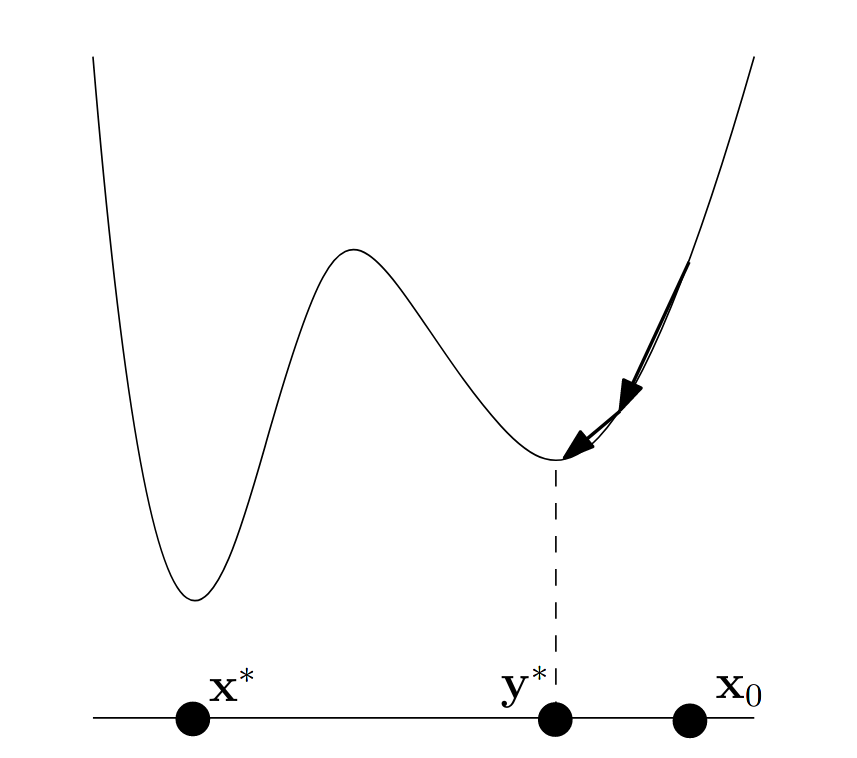
\includegraphics[height=0.8\textheight,keepaspectratio]{nonconvex.png}
  \end{figure}
\end{frame}


\begin{frame}
  \frametitle{Gradient Descent in the nonconvex world II}
  Even if there is a unique \textcolor{blue}{local} minimum (equal to the global minimum), we
  \begin{itemize}
    \item  may get stuck in a saddle point;
    \item run off to infinity;
    \item possibly encounter other bad behaviors.
  \end{itemize}
  \begin{figure}[ht]
    \centering
    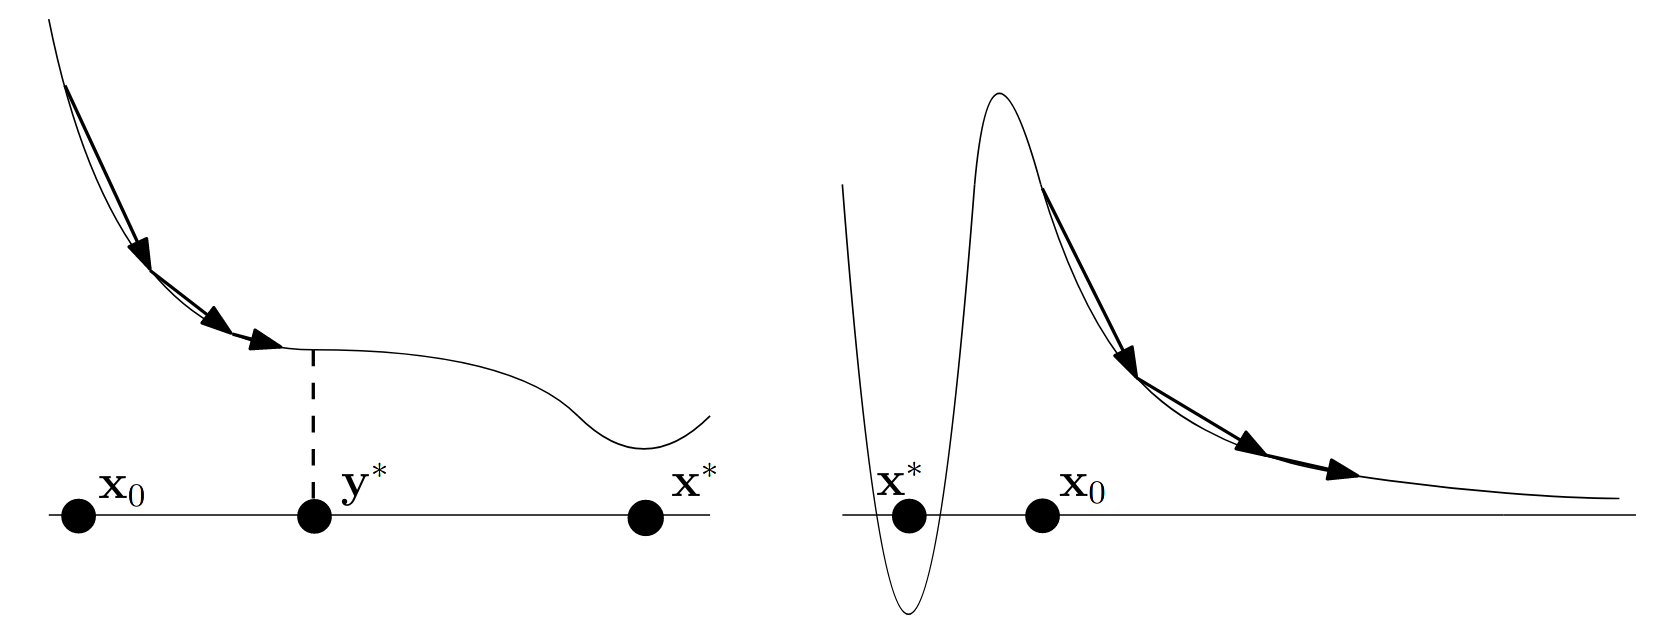
\includegraphics[width=\textwidth,height=\textheight,keepaspectratio]{nonconvex2}
  \end{figure}
\end{frame}


\begin{frame}
  \frametitle{Gradient Descent in the nonconvex world III}
  \begin{itemize}
    \item Often, we observe good behavior in practice.
    \item Theoretical explanations many times missing.
    \item Under favorable conditions, we sometimes can say something useful about
  the behavior of GD.
  \end{itemize}
\end{frame}


\section{Theory}%
\label{sec:}

\begin{frame}
  \frametitle{Smooth (but not necessarily convex) functions}
  \textbf{Recall}: A differentiable $f : \R^d \to \R$ is $L$-smooth over a convex set $X$ if
  \begin{equation}
    f(y) \le f(x) + \langle \nabla f(x), y- x \rangle + \frac{L}{2} \Vert y-x \Vert^2, \quad \forall x,y \in X.
  \end{equation}
  \begin{figure}[ht]
    \centering
    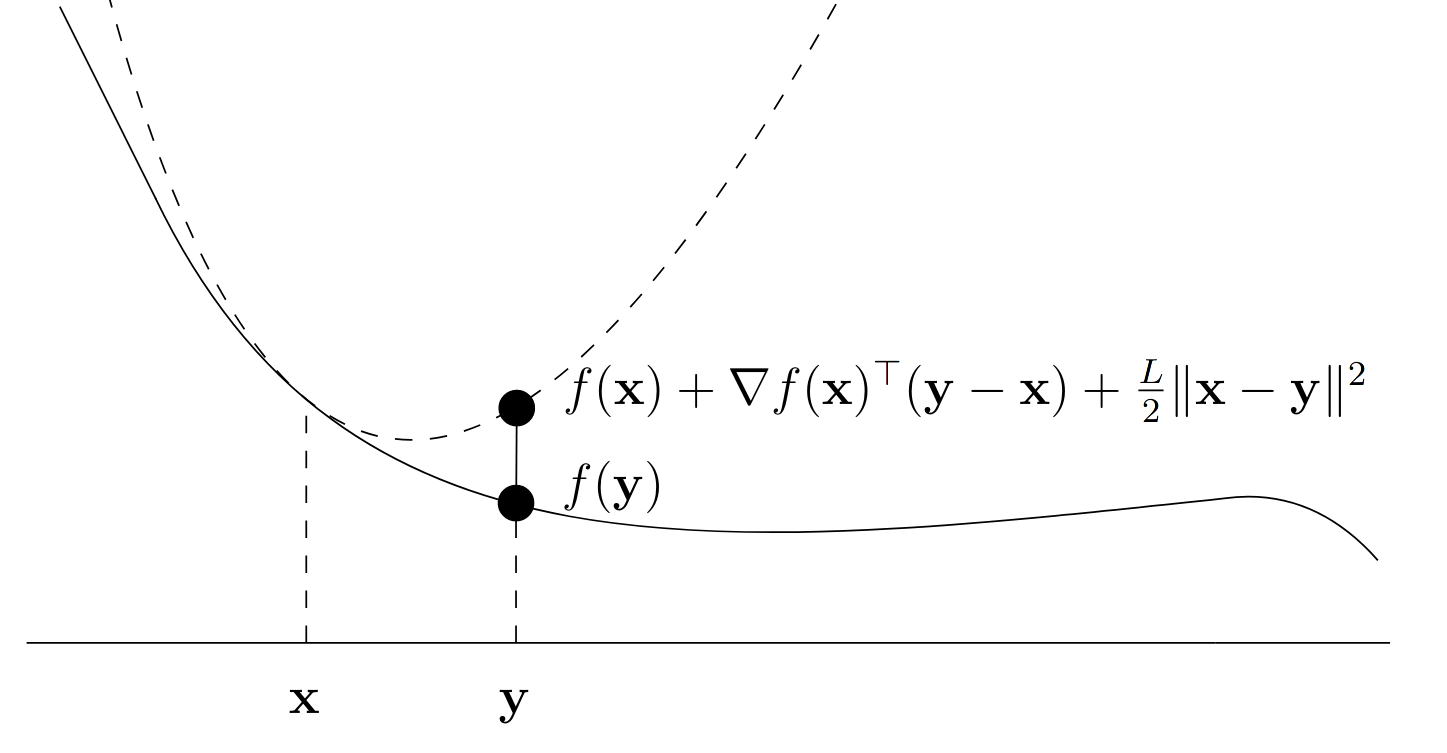
\includegraphics[height=0.65\textheight,keepaspectratio]{smoothness_no_convex}
  \end{figure}
\end{frame}


\begin{frame}
  \frametitle{Bounded Hessians $\Rightarrow$ smooth}
  \begin{lemma}%
    Let $f: \R^d \to \R$ be twice differentiable and
    \begin{equation}
      \Vert \nabla^2 f(x) \Vert \le L
    \end{equation}
    where $\Vert \cdot \Vert$ is spectral norm. Then $f$ is $L$-smooth
  \end{lemma}

  Examples:
  \begin{itemize}
    \item all quadratic functions $f(x)= x^T Ax + b^T x + c$
    \item $f(x) = \sin (x)$ (many global minima)
  \end{itemize}
\end{frame}


\begin{frame}
  \frametitle{Gradient descent on smooth functions}
  \begin{minipage}{0.5\textwidth}
  Will prove: $\Vert \nabla f(x_k) \Vert^2 \to 0$ \ldots \\
  \ldots at the \textbf{same rate} as \\
  $f(x_k) -f(x^*) \to 0$ in the convex case.
  \begin{itemize}
    \item $f(x_k) -f(x^*)$ itself may not converge to 0 in the nonconvex case:
  \end{itemize}
  \end{minipage}
  \begin{minipage}{0.45\textwidth}
    \begin{figure}[ht]
      \centering
      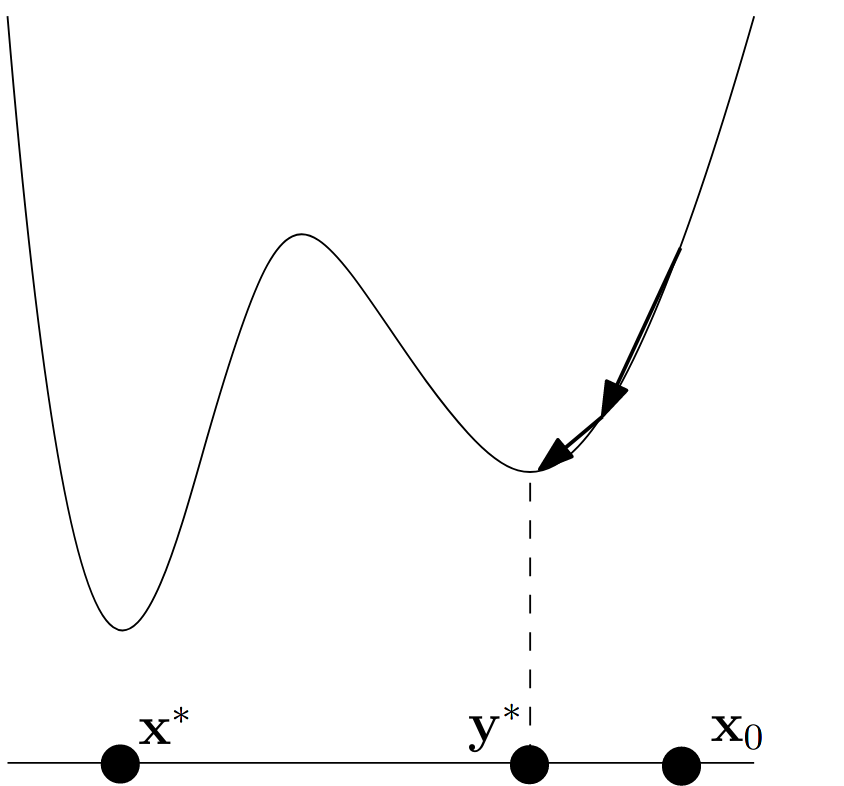
\includegraphics[height=0.7\textheight,keepaspectratio]{nonconvex_func}
    \end{figure}
  \end{minipage}
\end{frame}


\begin{frame}
  \frametitle{What does $\Vert \nabla f(x_k) \Vert^2\to 0$ mean?}
  \begin{itemize}
    \item May or \textcolor{blue}{may not} mean convergence to a critical point $\nabla f(y^*) =0$
    \item critical point might not be even local minimum
  \end{itemize}

  \begin{figure}[ht]
    \centering
    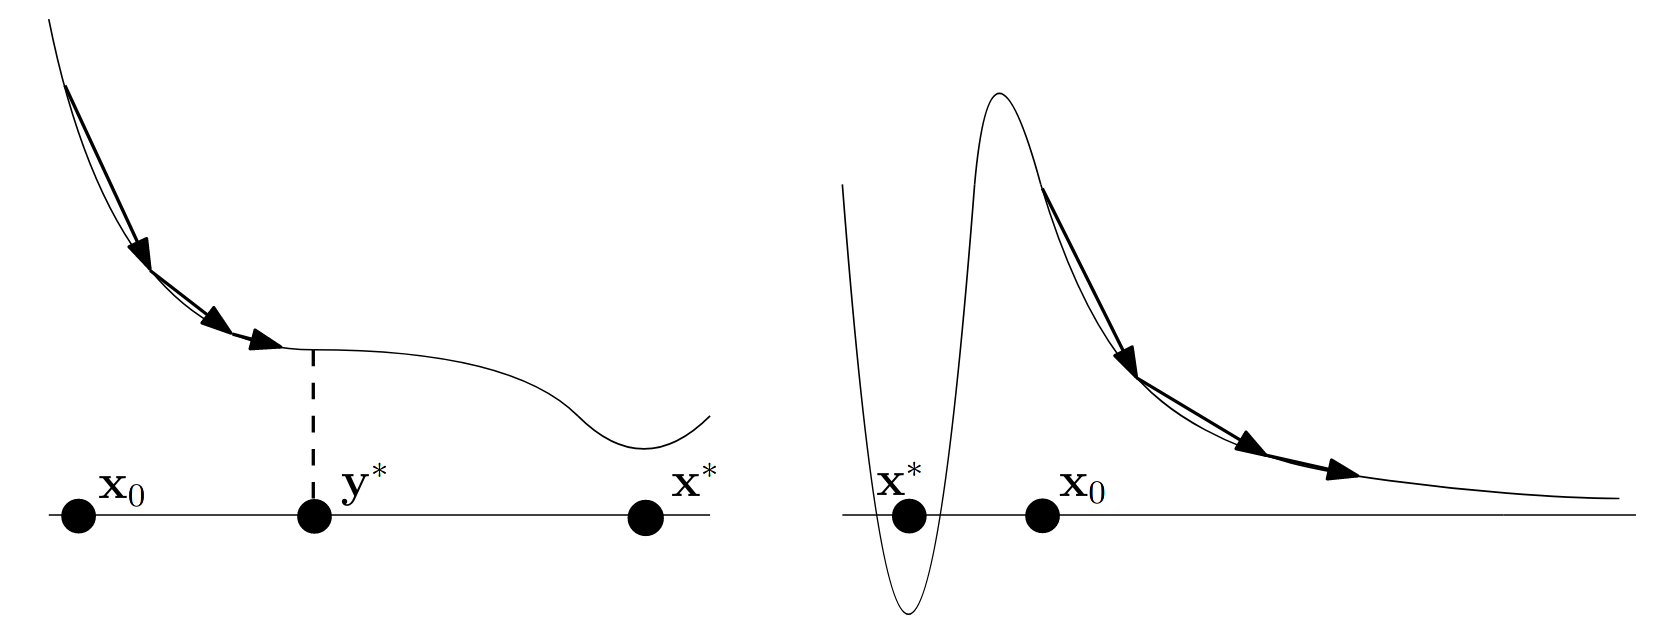
\includegraphics[width=\textwidth,height=\textheight,keepaspectratio]{nonconvex2}
  \end{figure}
\end{frame}


\begin{frame}
  \frametitle{Gradient descent on smooth (not necessarily convex) functions}

  \begin{theorem}
    Let $f : \R^d \to \R$ be $L$-smooth with a global minimum $x^*$. \\
    Choosing stepsize $\alpha := \frac{1}{L}$ gradient descent yields
    \begin{equation}
      \frac{1}{K} \sum_{k=0}^{K-1} \Vert \nabla f(x_k) \Vert^2 \le \frac{2L}{K} \big(f(x_0) - f(x^*)\big).
    \end{equation}
  \end{theorem}
  In particular, same bound hold for ``best'' iterate
  \begin{equation}
    \min_{0\le k \le K-1} \Vert \nabla f(x_k) \Vert^2 \le \frac{2L}{K} \big(f(x_0)-f(x^*)\big)
  \end{equation}
  and \textcolor{purple}{(prove this --- see exercises)}
  \begin{equation}
    \lim_{k \to \infty} \Vert \nabla f(x_k) \Vert^2 = 0.
  \end{equation}
\end{frame}


\begin{frame}
  \frametitle{Gradient descent on smooth  functions II: Proof}

  \textbf{Smoothness} gives:
  \begin{equation}
    f(y) \le f(x) + \langle \nabla f(x), y- x \rangle + \frac{L}{2} \Vert y-x \Vert^2.
  \end{equation}
  Use $y=x_{k+1}$ and $x=x_k$ to obtain
  \begin{equation}
    f(x_{k+1}) \le f(x_k) + \langle \nabla f(x_k), - \alpha \nabla f(x_k) \rangle + \frac{L \alpha^2}{2} \Vert \nabla f(x_k) \Vert^2.
  \end{equation}
  to obtain \textcolor{blue}{sufficient decrease:}
  \begin{equation}
    f(x_{k+1}) \le f(x_k) - \frac{1}{2L} \Vert \nabla f(x_k) \Vert^2.
  \end{equation}
\end{frame}


\begin{frame}
  \frametitle{Proof II}
  \textbf{Sufficient decrease:}
  \begin{equation}
    \frac{1}{2L} \Vert \nabla f(x_k) \Vert^2 \le f(x_k) - f(x_{k+1}).
  \end{equation}
  Sum up from $k=0, 1, \dots, K-1$ to get
  \begin{equation}
      \frac{1}{2L}\sum_{k=0}^{K-1} \Vert \nabla f(x_k) \Vert^2 \le f(x_0) - f(x_{k}) \le f(x_0) - f(x^*).
  \end{equation}
  Multiply by $2L/K$ to get the statement of the theorem.\qedhere
\end{frame}


\begin{frame}
  \frametitle{No overshooting}
  Under the \textbf{smoothness} assumption and \textbf{appropriate stepsize} $\alpha \le 1/L$,\\
  GD cannot pass a critical point:
  \begin{figure}[ht]
    \centering
    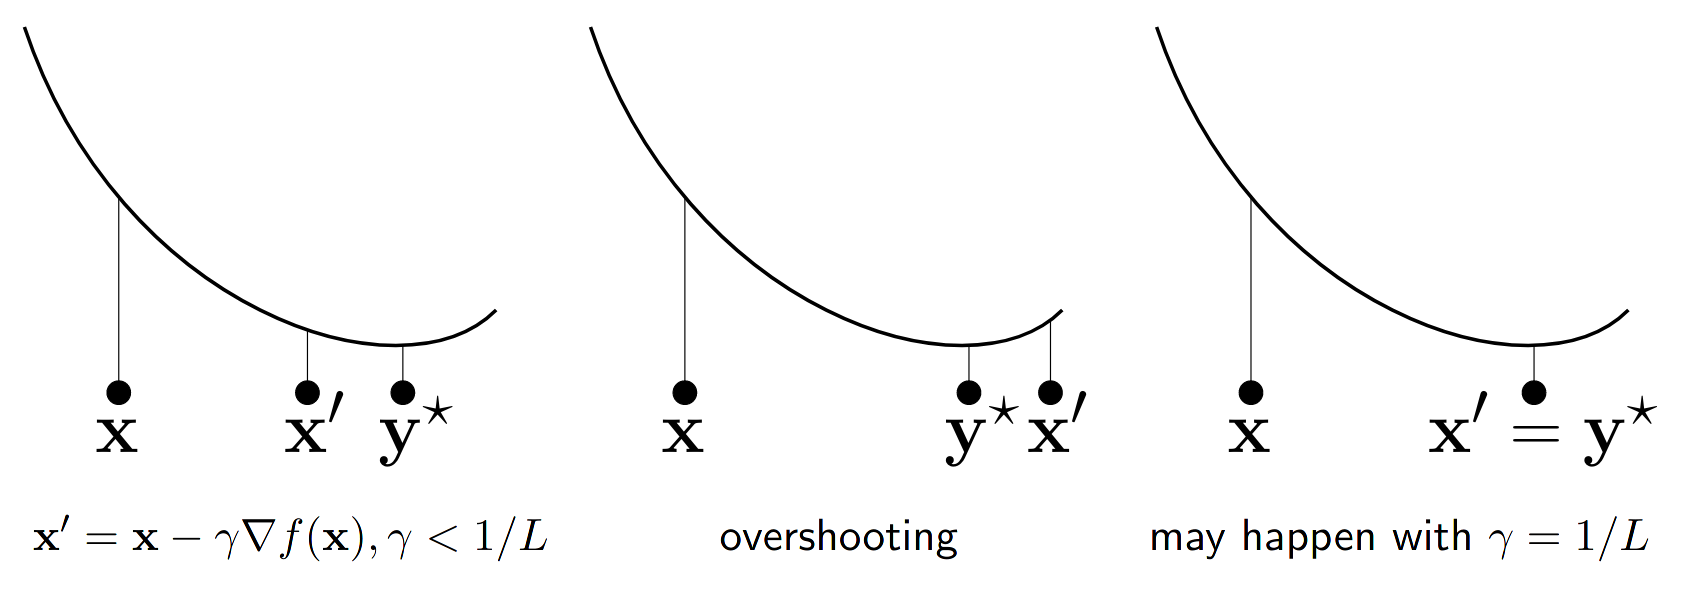
\includegraphics[width=\textwidth,height=\textheight,keepaspectratio]{no_overshooting}
  \end{figure}
\end{frame}


\section{GD for linear networks}%
\label{sec:}

\begin{frame}
  \frametitle{Trajectory Analysis}

  Even if the ``landscape'' (graph) of a nonconvex function has local minima, saddle
  points, and flat parts, gradient descent may avoid them and still converge to a global
  minimum.\medskip


  For this, one needs a \textbf{good starting point} and some theoretical understanding of what
  happens when we start there — this is trajectory analysis.

\end{frame}


\begin{frame}
  \frametitle{Linear models with several outputs}
  Recall: Learning linear models
  \begin{itemize}
    \item $n$ inputs $x_1,\dots,x_n$, where each input $x_i \in \R^d$
    \item $n$ outputs $y_1,\dots,y_n \in \R$
    \item Hypothesis (after centering / no bias):
          \begin{equation}
            y_i \approx w^T x_i ,
          \end{equation}
          for a weight vector $w = (w_1,...,w_d) \in \R^d$ to be learned.
  \end{itemize}

  Now more than one output value:
  \begin{itemize}
    \item $n$ outputs $y_1,\dots,y_n$, where each output $y_i \in \R^m$
    \item Hypothesis:
          \begin{equation}
            y_i \approx W x_i,
          \end{equation}
          for a weight matrix $W \in \R^{m\times d}$ to be learned.
  \end{itemize}
\end{frame}


\begin{frame}
  \frametitle{Minimizing the least squares error}

  Compute
  \begin{equation}
    W^* = \argmin_{W\in \R^{m\times d}} \sum_{i=1}^{n} \Vert W x_i - y_i \Vert^2.
  \end{equation}

  \begin{itemize}
    \item $X \in \R^{d \times n}$: matrix whose columns are the $x_i$
    \item $Y \in \R^{m \times n}$: matrix whose columns are the $y_i$
  \end{itemize}
  Then
  \begin{equation}
    W^* = \argmin_{W\in \R^{m\times d}} \sum_{i=1}^{n} \Vert W x_i - y_i \Vert_F^2.
  \end{equation}
  where $\Vert A \Vert_F = \sqrt{\sum_{i,j} a_{i,j}}$ is the Frobenius norm of a matrix $A$.\\
  \textcolor{gray}{Frobenius norm of A = Euclidean norm of \texttt{vec(A)} (``flattening'' of A).}

\end{frame}


\begin{frame}
  \frametitle{Minimizing the least squares error II}
  \begin{equation}
    W^* = \argmin_{W\in \R^{m\times d}} \Vert W X - Y \Vert_F^2
  \end{equation}
  \begin{minipage}{0.5\textwidth}
  \begin{itemize}
    \item global minimum of a convex quadratic function $f(W)$.
    \item To find $W^*$, solve $\nabla f(W)=0$ (system of linear equations)
    \item $\Leftrightarrow$ training a linear neural network with \textbf{one layer} under least squares loss.
  \end{itemize}
  \end{minipage}
  \begin{minipage}{0.45\textwidth}
    \begin{figure}[ht]
      \centering
      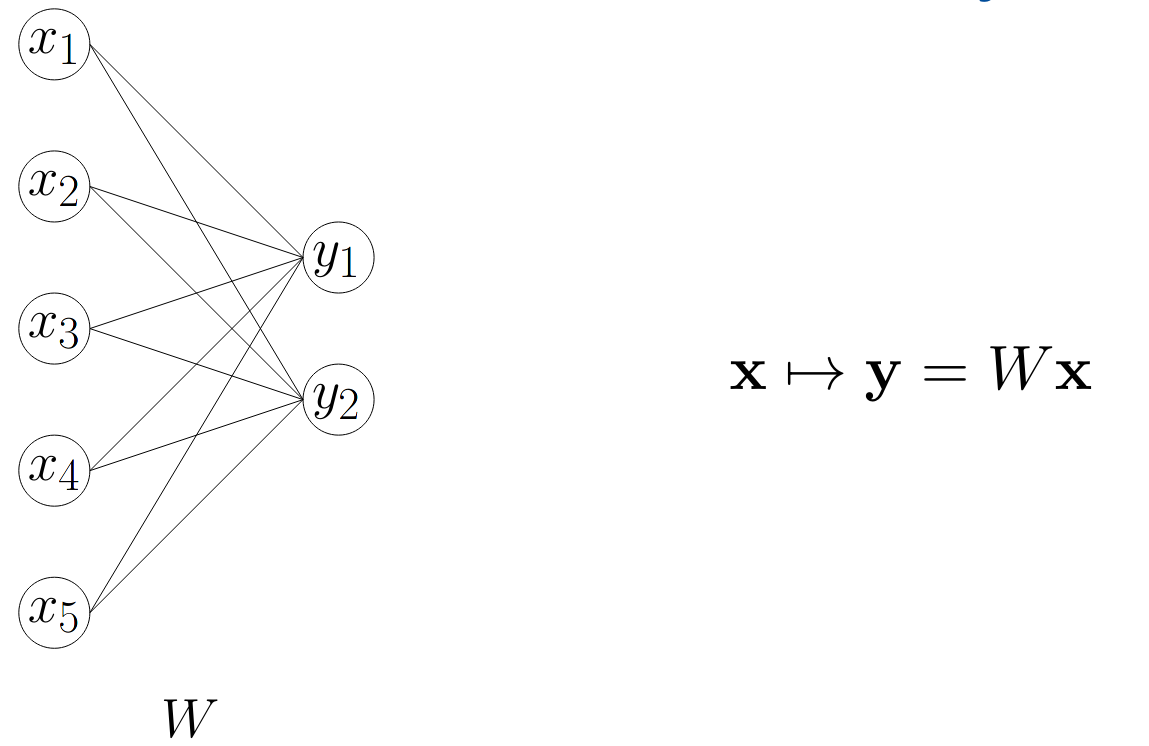
\includegraphics[height=0.6\textheight,keepaspectratio]{one-layer-linear-network}
    \end{figure}
  \end{minipage}
\end{frame}

\begin{frame}
  \frametitle{Deep linear neural networks}
  \begin{figure}[ht]
    \centering
    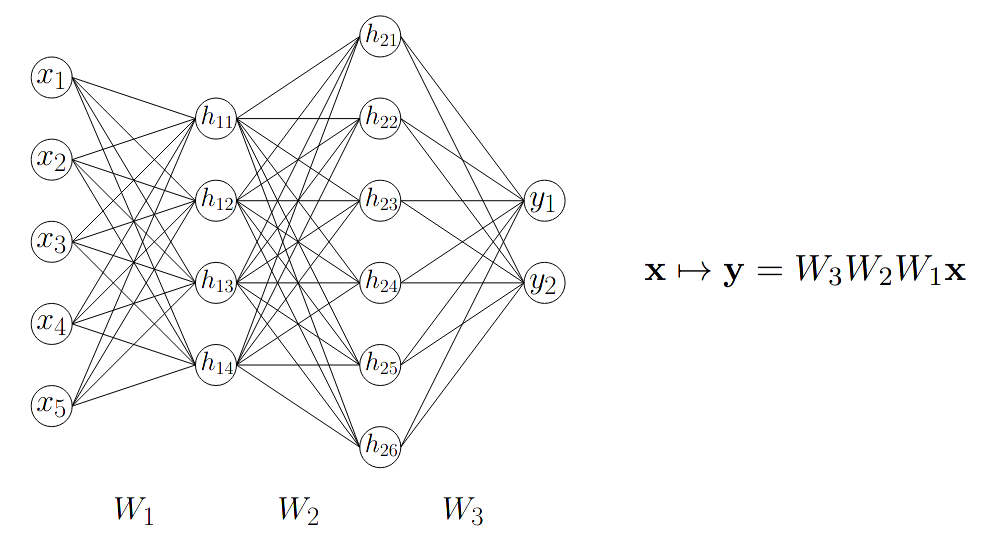
\includegraphics[height=0.6\textheight,keepaspectratio]{deep-linear-network}
  \end{figure}
  \textcolor{blue}{\textbf{Not more expressive}}:
  \begin{equation}
    x \mapsto W_3 W_2 W_1 x \Leftrightarrow x \mapsto Wx, \quad \text{for } W := W_3 W_2 W_1
  \end{equation}
\end{frame}


\begin{frame}
  \frametitle{Training deep linear neural networks}
  With $\ell$ layers:
  \begin{equation}
    W^* = \argmin_{W_1, W_2, \dots,  W_\ell} \Vert W_1 W_2 \cdots W_\ell X - Y \Vert_F^2
  \end{equation}
  \textcolor{blue}{\textbf{Nonconvex}} function for $\ell > 1$.

  Playground to understand why training deep neural networks with gradient descent works.

  Here: all matrices are $1 \times 1$, $W_i = x_i$, $X=1$, $Y = 1$, $\ell = d$
  $\Rightarrow f: \R^d \to \R$,
  \begin{equation}
    f(x) := \frac12 {\left(\prod_{j=1}^d x_j - 1\right)}^2 .
  \end{equation}

  Toy example in our simple playground
\end{frame}


\begin{frame}
  \frametitle{A simple nonconvex function}
  Nonconvex level sets: $f(x)= \frac12 {\left( \prod_j x_j \right)}$. \\
  \textcolor{gray}{Dimensions is fixed so we ignore it.}

  \begin{figure}[ht]
    \centering
    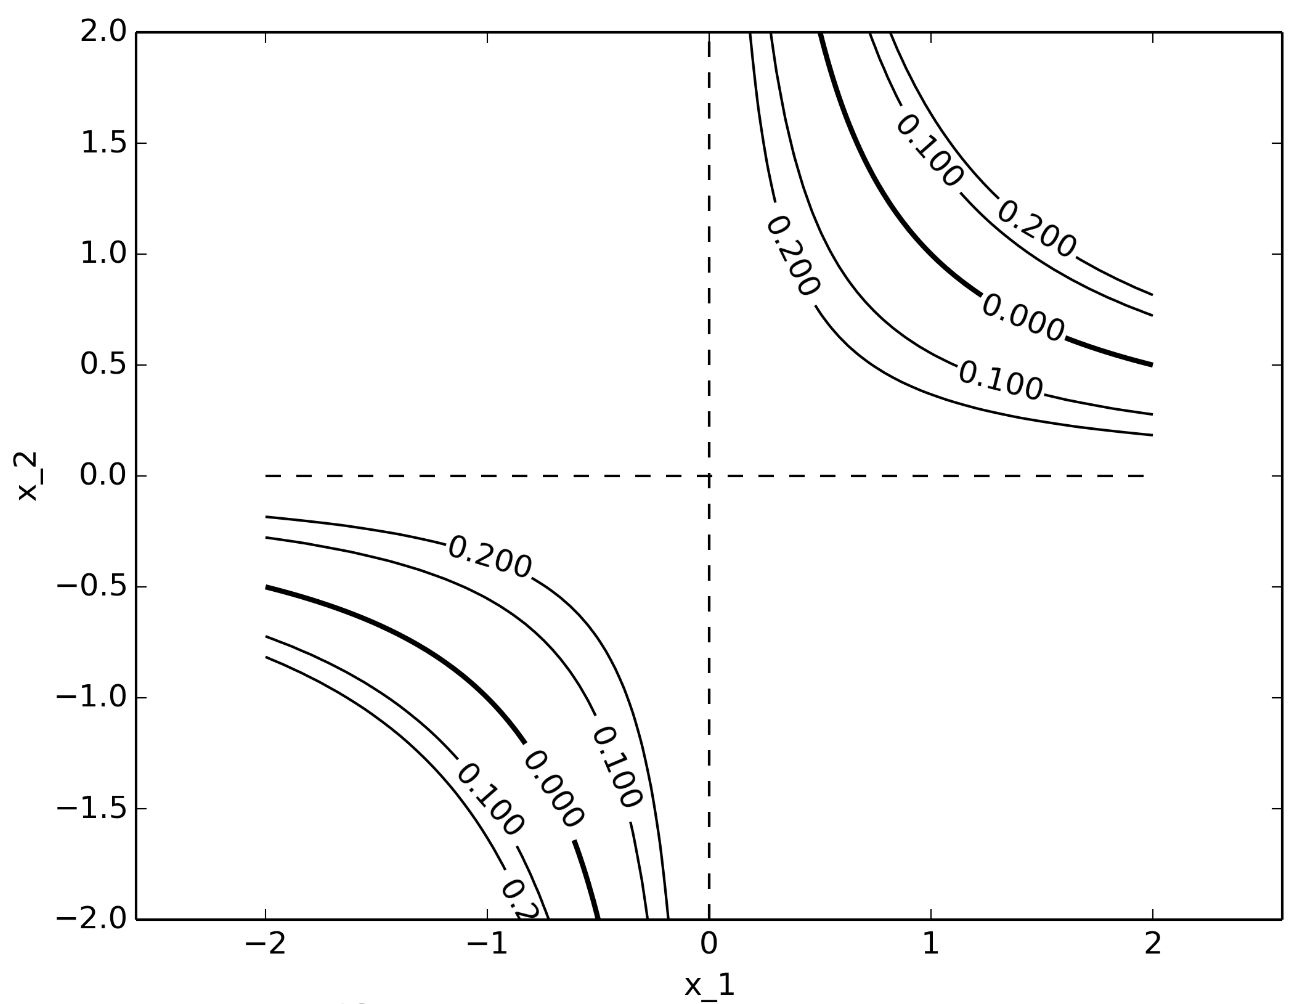
\includegraphics[height=0.6\textheight,keepaspectratio]{linear-network-toy}
  \end{figure}
\end{frame}


\begin{frame}
  \frametitle{Gradient and critical points}

  \begin{equation}
    \nabla f(x) = \left( \prod_j x_j \right) \left( \prod_{j\neq1} x_j, \cdots, \prod_{j\neq d}x_j \right).
  \end{equation}
  \begin{minipage}{0.5\textwidth}
    \begin{figure}[ht]
      \centering
      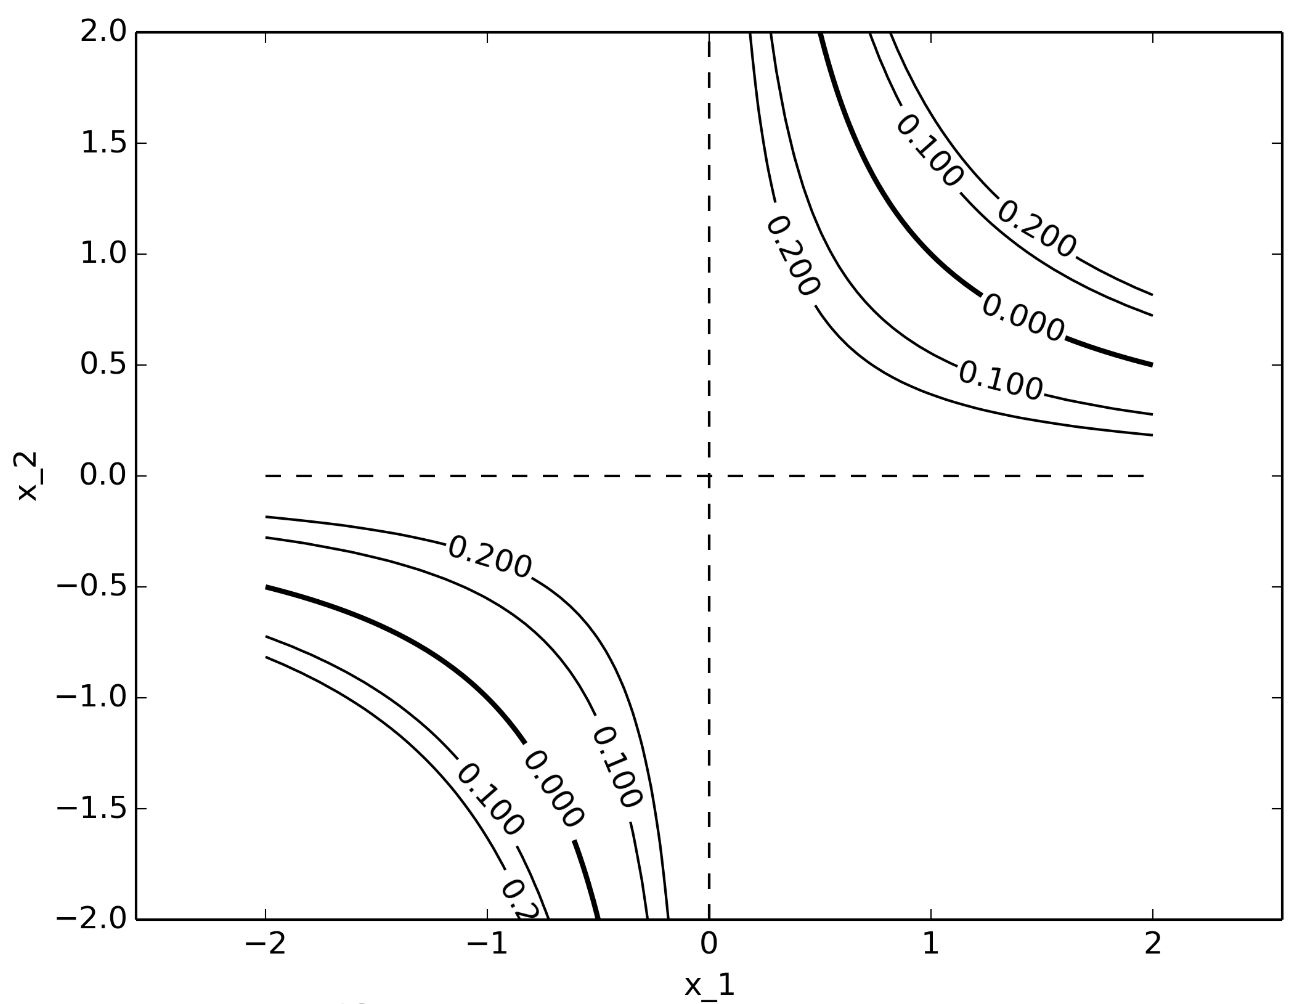
\includegraphics[width=\textwidth,keepaspectratio]{linear-network-toy}
    \end{figure}
  \end{minipage}
  \begin{minipage}{0.45\textwidth}
    Critical points ($\nabla f(x) = 0$) are either:
    \begin{itemize}
      \item global minima: if $\prod_j x_j = 1$
            \begin{itemize}
              \item $d=2$: hyperbola
            \end{itemize}
      \item saddle point: if at least two of $x_j$ are zero
            \begin{itemize}
              \item $d=2$: only the origin $(0,0)$
            \end{itemize}
    \end{itemize}
  \end{minipage}
\end{frame}


\begin{frame}
  \frametitle{Negative gradient directions}
  \begin{figure}[ht]
    \centering
    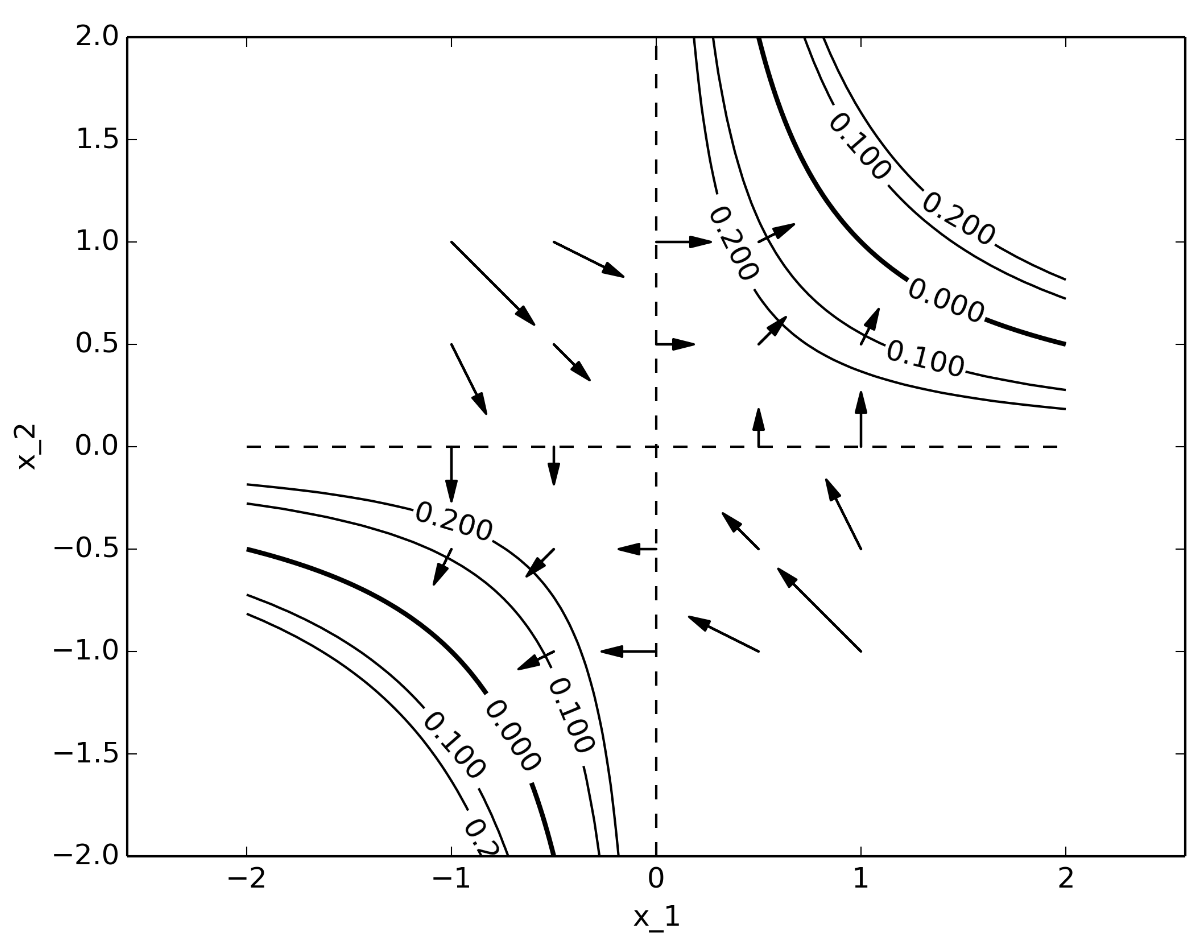
\includegraphics[height=0.8\textheight,keepaspectratio]{toy-example-neg-grad-directions}
  \end{figure}
  Convergence to global minimum from almost everywhere.
\end{frame}


\begin{frame}
  \frametitle{Convergence analysis: Overview}
  Convergence of GD holds for any $d>1$ and from anywhere in $X=\{x: x> 0, \prod_j x_j \le 1\}$.
  \begin{itemize}
    \item $f$ is not smooth over $X$.
          But is smooth along the trajectory: For suitable $L$ we still get
          \begin{equation}\tag{SD}
            \label{eq:sd}
            f(x_{k+1}) = f(x_k) - \frac{1}{2L} \Vert \nabla f(x_k) \Vert^2.
          \end{equation}
    \item saddle points have (at least two) zero entries $\Rightarrow$ function value $\ge$ $1/2$.
    \item any starting point $x_0 \in X$ has $f(x_0) < 1/2$
    \item cannot converge to saddle points through~\eqref{eq:sd}
  \end{itemize}

  Still does not imply convergence to global minimum:
  \begin{itemize}
    \item Sublevel sets are unbounded: GD can run off to $\infty$
  \end{itemize}

\end{frame}


\begin{frame}
  \frametitle{Convergence analysis: Overview II}

  For $x> 0, \prod_j x_j \ge 1$, we can also show convergence: \\
  $\Rightarrow$ convergence anywhere in the interior of the positive orthant $\{x: x> 0\}$.

  For this, recall that
  \begin{equation}
    \nabla f(x) = \left( \prod_j x_j \right) \left( \prod_{j\neq1} x_j, \cdots, \prod_{j\neq d}x_j \right).
  \end{equation}

  \begin{itemize}
    \item since $\prod_j x_j \ge 1$ then $\nabla f(x) \ge 0$
    \item which implies that $x_{1} \le x_0$ (componentwise)
    \item iterates remain in a bounded set $\Rightarrow$ smoothness on this set
  \end{itemize}

\end{frame}


\begin{frame}
  \frametitle{}
  \begin{definition}
    Let $x > 0$ (componentwise), and let $c \ge 1$. $x$ is called $c$-balanced if $x_i \le cx_j$ for all $1 \le i, j \le d$.
  \end{definition}

  \begin{theorem}
    Let $c\ge 1$ and $\delta> 0$ such that $x^0 > 0$ is $c$-balanced with $\delta \le \prod_j x^0_j < 1$. Choosing the stepsize
    \begin{equation}
      \gamma = \frac{1}{3d c^2}
    \end{equation}
    gradient descent satisfies
    \begin{equation}
      f(x^k) \le {\left( 1- \frac{\delta^2}{3 c^4} \right)}^k f(x^0).
    \end{equation}
  \end{theorem}
\end{frame}


\begin{frame}
  \frametitle{Discussion}

  \begin{itemize}
    \item Error converges to 0 exponentially fast.
    \item But there's a catch: Consider $x^0 = (1/2, \dots, 1/2)$. Then $\delta \le \prod_j x^0_j = 2^{-d}$
    \item Decrease in function value per step by factor
          \begin{equation}
            \left( 1- \frac{1}{3 4^d} \right).
          \end{equation}
    \item Contraction coefficient depends \textit{exponentially bad on dimension}
    \item polynomial runtime: must start at distance $\mathcal{O}(1/\sqrt{d})$ from optimality.
  \end{itemize}
\end{frame}


\section{Matrix completion}%
\label{sec:}

\begin{frame}
  \frametitle{Matrix completion}

  is the problem of recovering a \textbf{low rank} ($r \ll d$) matrix $M \in \R^{d\times d}$ \\
  from \textcolor{blue}{partially observed entries}:
  \begin{block}{}
    \textbf{Application: Netflix problem}
  \end{block}
  \begin{align}
    \min_{X\in \R^{d\times d}} &\, \rank(X) \\
    \text{subject to } & X_{i,j} = M_{i,j}, \quad \forall i,j \in \Omega
  \end{align}
  But rank is \textbf{not continuous}\ldots
\end{frame}


\begin{frame}
  \frametitle{Convex matrix completion}

  Typically \textbf{convex} reformulations are considered via the\\
  \textbf{Nuclear norm} (sum of singular values)
  \begin{align}
    \min_{X\in \R^{d\times d}} &\, \Vert X \Vert_* := \sum_j \sigma_j(X) \\
    \text{subject to } & X_{i,j} = M_{i,j}, \quad \forall i,j \in \Omega
  \end{align}
  \begin{itemize}
    \item strong theoretical guarantees
    \item can be expensive
          \begin{itemize}
            \item $\mathcal{O}(d^3)$ running time
            \item $\mathcal{O}(d^2)$ memory.
          \end{itemize}
  \end{itemize}
\end{frame}


\begin{frame}
  \frametitle{Nonconvex matrix completion}
  Can be cast in the bilinear $X \approx U V^T$ form which gives:
  \begin{align}
    \min_{U, V \in \R^{d\times r}} &\, \sum_{i,j \in \Omega} \Vert {(UV^T)}_{i,j} - M_{i,j} \Vert^2.
  \end{align}
  \begin{itemize}
    \item many global minima
    \item if $UV^T = M$ then $(UQ){(VQ)}^T = M$ for any orthonormal matrix $Q$ \\
          \textcolor{gray}{orthonormal: $Q Q^T = \Id$}
  \end{itemize}

  \begin{block}{}
    \center
    No spurious local minima!
  \end{block}
  Can often be efficiently solved by GD or alternating minimization.

\end{frame}



\end{document}
